\section{Das Analyseklassendiagramm}
Aufgrund der Use-Case-Diagramme im Kapitel \ref{Use Case Diagramme} und der Wireframes im Kapitel \ref{Wireframes} wurde nun ein Klassendiagramm erstellt, welches die Grundlegende Struktur der App verdeutlichen soll. Hierbei wurde bewusst auf Methoden und Klassenvariablen verzichtet um die \"Ubersichtlichkeit des Diagramms zu gew\"ahrleisten.


\begin{figure}[!ht]
\centering
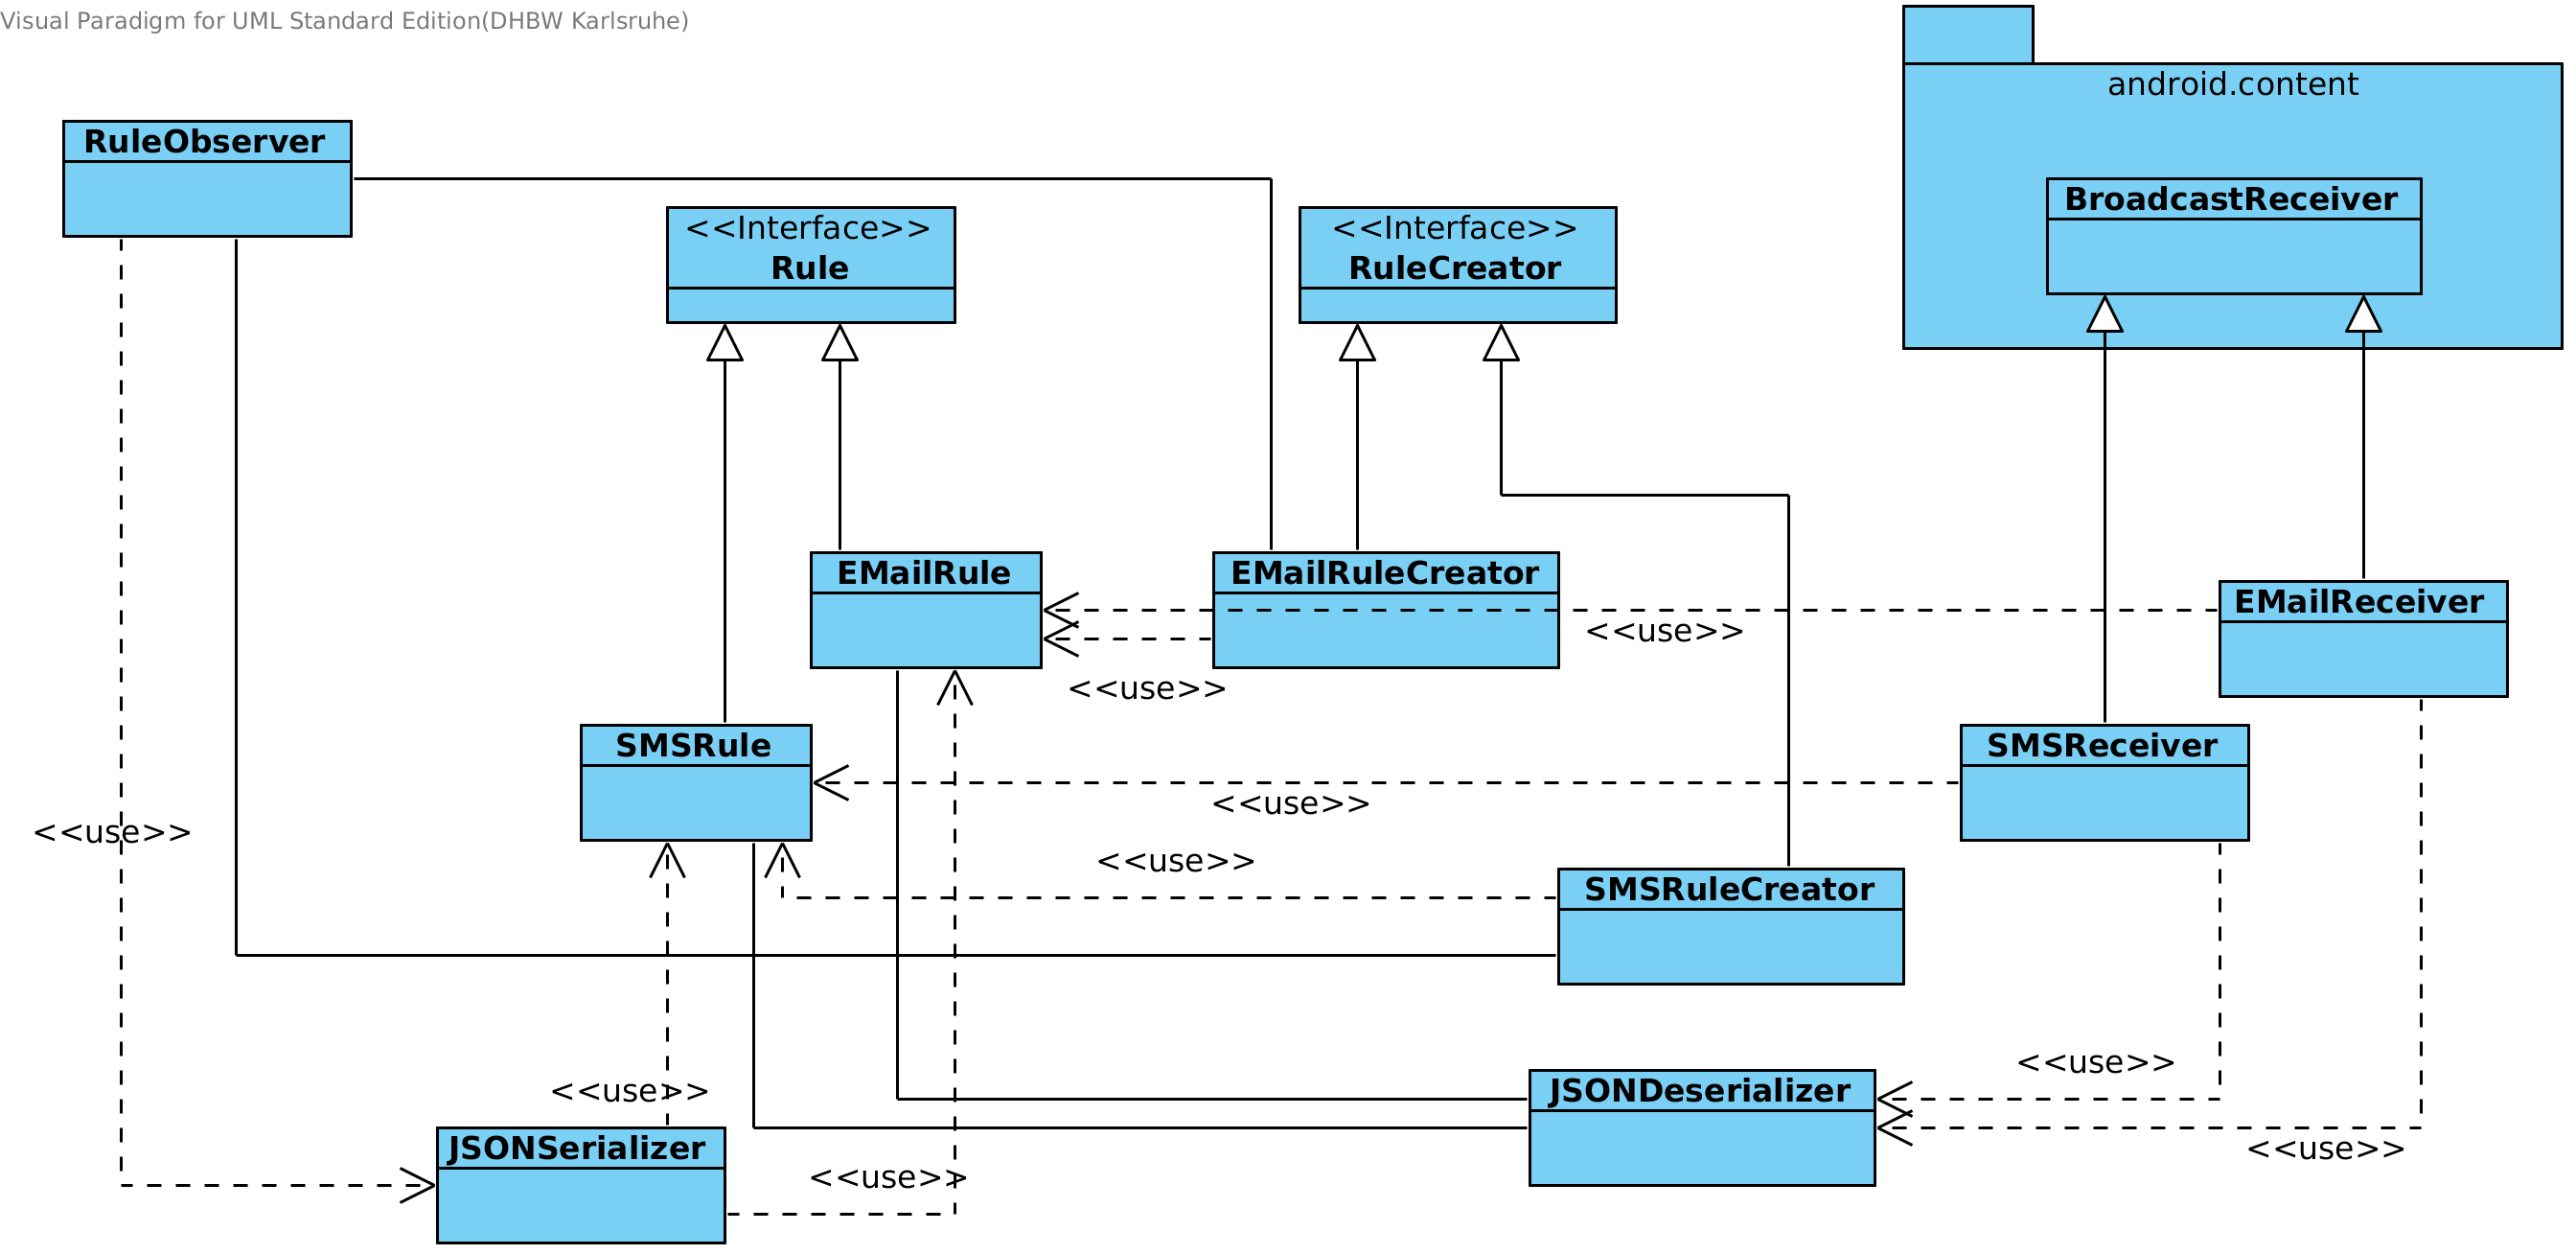
\includegraphics[width=16cm]{Bilder/AKD.png}
\caption{Analyseklassendiagramm der App}
\label{AKD}
\centering
\end{figure}